\documentclass[border={7pt 0pt 7pt 0pt},varwidth]{standalone}
\usepackage{amsmath}
\usepackage[dvipsnames]{xcolor}%colors
\usepackage{tikz-cd,tikz-3dplot} 
\usepackage{diagbox}
\usepackage{makecell}
\usepackage{adjustbox}
\usepackage{multirow}
\usepackage[width=0.5,tiewidth=0.7]{strands}
\usepackage{array}


\newcommand{\fakestar}{*}

% https://tex.stackexchange.com/questions/372642/looking-for-symbol-fire
\usepackage{fontspec}
\newfontfamily\emojifont{OpenSansEmoji} % https://github.com/MorbZ/OpenSansEmoji
\DeclareTextFontCommand{\emoji}{\emojifont}
\begin{document}
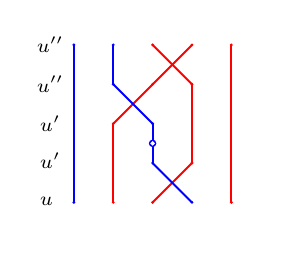
\begin{tikzpicture}[baseline=(current bounding box)]
                 \node at (-0.3,0.06) {$\scriptstyle u\phantom{'}$};
                 \node at (2.3,0.06) {$\phantom{\scriptstyle u'}$};
                 \node at (-0.3,0.53) {$\scriptstyle u'$};
                 \node at (-0.3,1) {$\scriptstyle u'$};
                 \node at (-0.3,1.5) {$\scriptstyle u''$};
                 \node at (-0.3,2) {$\scriptstyle u''$};
%                 \node at (1,-0.15) {$\scriptstyle i$};
                 \node at (1.5,-0.15) {$\phantom{\scriptstyle i+1}$};
                 \tie[color=blue,bull=1,bulletie=0.01,style=solid]{{1,2},{1,0}}
                 \tie[color=red,bull=1,bulletie=0.01,style=solid]{{4,2},{3,1.5},{2,1},{2,0}}
                 \tie[color=red,bull=1,bulletie=0.01,style=solid]{{3,2},{4,1.5},{4,0.5},{3,0}}
                 \tie[color=blue,bull=1,bulletie=0.01,style=solid]{{2,2},{2,1.5},{3,1},{3,0.5},{4,0}}
                 \tie[color=red,bull=1,bulletie=0.01,style=solid]{{5,2},{5,0}} \tie[color=blue]{{3,0.75}}\tie[color=white,bulletie=0.02]{{3,0.75}}
\end{tikzpicture}


\end{document}